\section{Implementación y programación}\label{sec:implemetacion_y_programacion}

En esta sección vamos a explicar algunos de los detalles de implementación de aquellos componentes que creemos que es
interesante que sean introducidos.

\subsection*{Componente \textit{Generator}}

\subsubsection*{PDF To Text Processor}

Como puede verse en el siguiente extracto de código, el procesador \textbf{PDF To Text Processor} es simplemente un
envoltorio para \textbf{Pdf to Text}.

\lstinputlisting[language=PHP]{chapter/4/code/PdfToTextProcessor.php}

En la figura~\ref{fig:chapter_4.generator_component_pdf_to_text_processor} puede verse un esquema de este
comportamiento.

\begin{figure}[ht]
    \begin{center}
        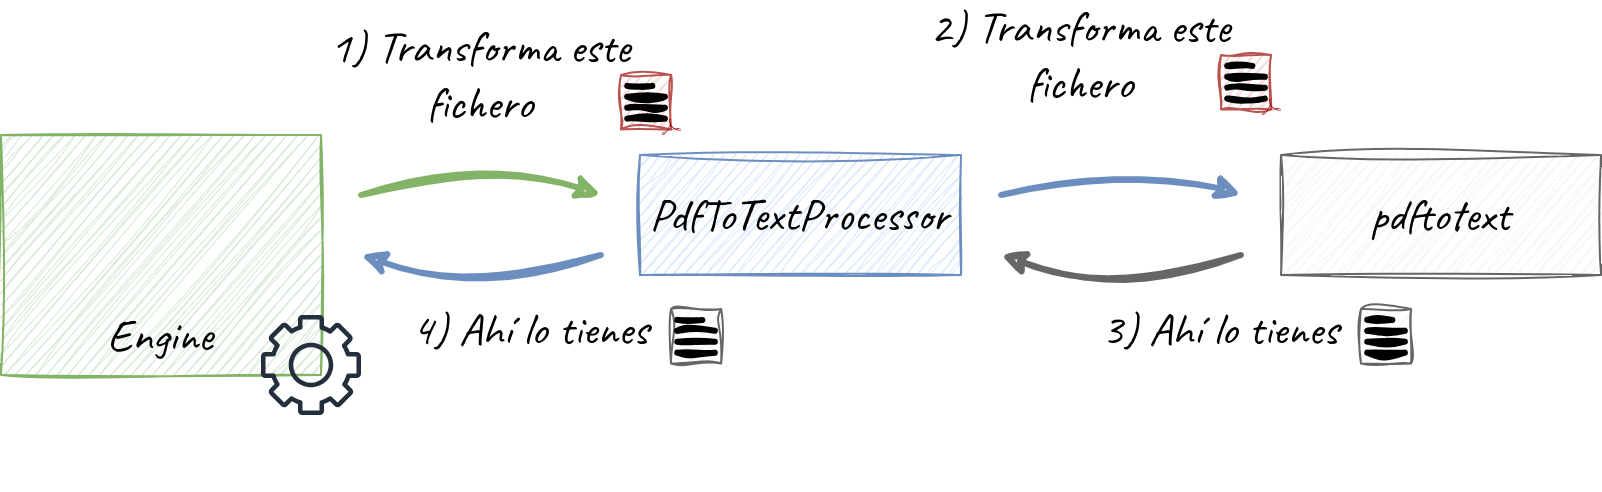
\includegraphics[width=\textwidth]{./chapter/4/images/chapter_4.generator_component_pdf_to_text_processor}
        \caption{Esquema de comunicación con pdftotext}
        \label{fig:chapter_4.generator_component_pdf_to_text_processor}
    \end{center}
\end{figure}

\subsection*{Componente \textit{Reader}}

\subsubsection*{Residential Lease Processor}

La implementación de este procesador es muy similar a la que hemos visto en el \textbf{PDF To Text Processor}, por lo
que no vamos a incluir ni el código ni un esquema de la comunicación.

Simplemente, indicaremos que se trata de enviar preguntas sobre un documento que previamente hemos convertido en texto
plano a un sistema LLM, en este caso utilizaremos el modelo
\textbf{ChatGPT 4}~\cite{https://platform.openai.com/docs/models/gpt-4}

Lo que si merece la pena es profundizar en los mensajes que se envían.

El primer intento de implementación se trató que el modelo respondiera con un XML. Para ello en la pregunta se le
facilitaría un XSD, con los tipos de datos y sus validaciones.
Sin embargo \textbf{ChatGPT 4} tiene limitaciones para trabajar con documentos XML, por lo que la implementación final
se realizó utilizando ejemplos JSON.

\lstinputlisting[language=PHP]{chapter/4/code/ResidentialLeaseAgreementProcessor.php}

Como puede verse en el ejemplo de código anterior, es vital ser muy preciso en cuanto a la información que se le
solicita y en cuanto al formato en el que se va a esperar la respuesta.
Para ello se le facilita un ejemplo con los tipos de datos de cada dato.

\subsubsection*{Vehicle Sale And Purchase Processor}

\subsubsection*{Caché}

La implementación de una caché en aplicaciones web es una técnica comúnmente utilizada para mejorar el rendimiento y la
eficiencia..

En este proyecto, la caché se ha utilizado específicamente para almacenar las peticiones HTTP realizadas, proporcionando
varias ventajas significativas, como el aumento de la velocidad de respuesta y la reducción de costos operativos..

Aunque en un entorno de producción la utilidad de esta caché podría ser limitada, en un entorno de desarrollo resulta
invaluable.

Esto se debe a que en desarrollo se trabaja principalmente con un conjunto de datos más pequeño y las peticiones se
repiten con frecuencia.

\subsection*{Registros}

El registro de logs es una parte crucial del monitoreo y mantenimiento de cualquier aplicación..

En este proyecto, se ha implementado un sistema de logging utilizando Monolog, una biblioteca de registro para PHP.

Además de los logs que almacena symfony por defecto, se han configurado 3 canales adicionales:

\begin{itemize}
    \item Generator: para los logs del componente generator.
    \item Reader: para los logs del componente reader.
    \item Http-Client: para el componente que realiza las peticiones HTTP.
\end{itemize}

Un canal es la forma en la que monolog, agrupa un conjunto de información para poderla filtrar y procesar adecuadamente.

Canal además se registra en dos ficheros diferentes

\begin{itemize}
    \item Log File format, es el formato estándar de ficheros de logs.
    \item Logstash format, es el estándar de la herramienta logstash.
\end{itemize}

\subsection*{Formato de ficheros por defecto}
El formato por defecto es adecuado para entornos de desarrollo o proyectos de pequeña envergadura. Siempre que estos
ficheros no sean demasiado grandes, se pueden trabajar a través de herramientas de línea de comandos como:

\begin{itemize}
    \item grep: Utilizado para buscar patrones específicos dentro de los archivos de logs.
    \item awk: Utilizado para procesar y analizar los logs de manera más compleja.
\end{itemize}

\subsection*{Sistema ELK}
Un sistema compuesto por Elasticsearch, Logstash y Kibana (ELK) es una solución centralizada de gestión de logs, que
permite una monitorización más avanzada de los mismos.
Está indicado en entornos de producción, donde la monitorización de logs sea una tarea importante..


Monitorización de logs a través de un sistema ELK

El sistema ELK se compone de tres componentes:

\begin{itemize}
    \item
    Logstash: Es una herramienta de procesamiento de datos que ingiere, transforma y envía datos a diversos destinos,
    siendo Elasticsearch uno de los más comunes.
    \item
    Elasticsearch: Es un motor de búsqueda y análisis de texto completo basado en Lucene. Permite almacenar, buscar y
    analizar grandes volúmenes de datos en tiempo real.
    \item Kibana: Es una herramienta de visualización de datos que trabaja en conjunto con Elasticsearch. Permite a los
    usuarios crear gráficos y dashboards interactivos para visualizar y analizar los datos de logs almacenados en
    Elasticsearch.
\end{itemize}

\colorbox{color_highlight}{@TODO: @marlene:}
Vale, veo que si usas el LLM de chatgpt. Eso es algo que no me había quedado claro de la memoria. Sin embargo, aún
no
tengo del todo claro qué generas a partir del PDF que recibes. Puedes ejecutar tu herramienta con un contrato? Estás
usando el LLM para extraer los datos del contenido del PDF? Otra pregunta, qué modelo de chatgpt estás usando? Y
puedes
mandar el prompt que usaste?